%\documentclass[8pt, handout]{beamer}
%\usepackage{pgfpages} 								%Для распечатки
%\pgfpagesuselayout{2 on 1}[a4paper,border shrink=10mm]

\documentclass[8pt]{beamer}

\usepackage[english,russian]{babel}
\usepackage[utf8]{inputenc}
\usepackage{mflogo}
\usepackage{amsmath,amsfonts,amssymb}
\usepackage{euscript}
\usepackage{graphicx}
\usepackage{xcolor}
\usepackage{transparent}

\newcommand{\grad}{\mathrm{grad\,}}
\newcommand{\pp}[2]{\frac{\partial #1}{\partial #2}}
\newcommand{\ds}{\displaystyle}


\beamertemplatenavigationsymbolsempty

\usetheme{EastLansing}
\setbeamercovered{transparent}


\title[Функции многих переменных]{Математический анализ\\ Тема 6: Функции многих переменных}
\author[Выборный Е. В.]{Выборный Евгений Викторович\\ email: evybornyi@hse.ru}
\date{Москва 2016} 


\makeatletter
\setbeamertemplate{footline}{
    \leavevmode%
    \hbox{%
    \begin{beamercolorbox}[wd=.25\paperwidth, ht=2.5ex, dp=1ex, center]{author in head/foot}%
        \usebeamerfont{author in head/foot}%
        \insertshortauthor
    \end{beamercolorbox}%
    \begin{beamercolorbox}[wd=.5\paperwidth,ht=2.5ex,dp=1ex,center]{title in head/foot}%
        \usebeamerfont{title in head/foot}\insertshorttitle
    \end{beamercolorbox}%
    \begin{beamercolorbox}[wd=.25\paperwidth,ht=2.5ex,dp=1ex,right]{date in head/foot}%
        \usebeamerfont{date in head/foot}\insertshortdate{}\hspace*{2em}
        \insertframenumber{} / \inserttotalframenumber\hspace*{2ex}
    \end{beamercolorbox}}%
    \vskip0pt%
}
\makeatother

\makeatletter
\setbeamertemplate{title page}
{
\centering
 \usebeamerfont{author}\insertauthor
 \vfill
 \begin{beamercolorbox}[rounded=true,shadow=true,sep=8pt,center]{title}
  \usebeamerfont{title}\inserttitle
 \end{beamercolorbox}
\vfill
\centering
\insertdate\par
 \vskip0.2em
}
\makeatother

\begin{document}
%\parindent=1.5em %красная строка

\begin{frame}
\titlepage
\end{frame}

\begin{frame}{Пространство $\mathbb{R}^n$}
\begin{block}{Определение. Вещественное $n$-мерное пространство $\mathbb{R}^n$}
Множество упорядоченных наборов из $n$ действительных чисел называют {\bf вещественным $n$-мерным пространством} $\mathbb{R}^n$:
$$x=(x_1,\ x_2,\ldots,\ x_n)\in \mathbb{R}^n.$$
Эти наборы чисел из $\mathbb{R}^n$ называют точками или векторами. В $\mathbb{R}^n$ определена сумма векторов и операция умножения вектора на число:
$$x+y = (x_1,\ x_2,\ldots,\ x_n)+(y_1,\ y_2,\ldots,\ y_n) = (x_1+y_1,\ x_2+y_2,\ldots,\ x_n+y_n),$$
$$\alpha x = \alpha\cdot (x_1,\ x_2,\ldots,\ x_n) = (\alpha x_1,\ \alpha x_2,\ldots,\ \alpha x_n).$$
Определено понятие расстояния между точкам:
$$d(x,y) = \|x-y\| = \sqrt{(x_1-y_1)^2+\cdots+(x_n-y_n)^2}.$$
Выполнено неравенство треугольника:
$$\|x+y\|\le \|x\|+\|y\|.$$
\end{block}
\end{frame}

\begin{frame}{Шар в $\mathbb{R}^n$}
Ключевым понятием для определения сходимости в одномерном случае была $\varepsilon$-окрестность точки $a$. Определим аналогичные понятия в многомерном пространстве $\mathbb{R}^n$.

\begin{block}{Определение. Шар в $\mathbb{R}^n$}
{\bf Открытым шаром} в $\mathbb{R}^n$ с центром в точке $a$ и радиусом $r$ называют множество точек $x\in \mathbb{R}^n$, удовлетворяющих условию
$$\|x-a\|< r\ \iff\ (x_1-a_1)^2+\cdots+(x_n-a_n)^2 < r^2.$$
Иногда это множество называют $r$-окрестностью точки $a$, сохраняя обозначение $O_r(a)$. Тогда {\bf проколотой $r$-окрестностью} точки $a$, называют множество точек:
$$\dot O_r(a) = O_r(a)\setminus \{a\} = 
\left\{ x\in\mathbb{R}^n\mid 0<\|x-a\|<r \right\}.
$$ 
\end{block}
\begin{block}{Определение. Ограниченное множество}
Множество $A\subset\mathbb{R}^n$ называется {\bf ограниченным}, если $A$ полностью лежит в некотором шаре. В этом случае существует $R$ такое, что
$$\|x\|<R\quad \forall x\in A.$$
\end{block}
\end{frame}

\begin{frame}{Предел последовательности точек}

\begin{block}{Определение. Предел последовательности точек}
Говорят, что последовательность точек $\{x^{(k)}\}$, $x^{(k)}\in\mathbb{R}^n$ сходится к точке $y\in\mathbb{R}^n$, пишут~$x^{(k)}\to y$, если к нулю стремится расстояние между $y$ и $x^{(k)}$ при $k\to+\infty$:
$$\lim_{k\to+\infty} d(y,\ x^{(k)}) = 0.$$
Эквивалентные записи имеют вид:
$$\forall\varepsilon>0\ \exists N:\quad x^{(k)}\in O_\varepsilon(y) \quad \forall k\ge N.$$ 
$$\forall\varepsilon>0\ \exists N:\quad \|x^{(k)} -y\|<\varepsilon \quad \forall k\ge N.$$
Таким образом, последовательность точек стремится к $y$ тогда и только тогда, когда в любом открытом шаре с центром в точке $y$ лежит бесконечно много точек последовательности, а вне его --- лишь конечное число.
\end{block}
\begin{block}{Упражнение}
Докажите, что множество точек сходящейся последовательности является ограниченным.
\end{block}
\end{frame}

\begin{frame}{Предел последовательности точек}

\begin{block}{Предложение}
Сходимость последовательности точек $\{x^{(k)}\}$ к точке $y$ эквивалентна сходимости координат точек $x^{(k)} = ( x_1^{(k)},\ldots,x_n^{(k)})$ к координатам точки $y = (y_1,\ldots,y_n)$:
$$\lim_{k\to+\infty} x^{(k)} = y\quad \iff \quad 
\lim_{k\to+\infty}x_1^{(k)} = y_1,\ldots,\lim_{k\to+\infty}x_n^{(k)} = y_n.$$
\end{block}

\begin{block}{Доказательство}
Доказательство теоремы непосредственно следует из очевидных неравенств:
$$|x_j^{(k)} - y_j|\le \sqrt{(x^{(k)}_1-y_1)^2+\cdots+(x^{(k)}_n-y_n)^2} \le n\max_{1\le j\le n} |x_j^{(k)} - y_j|.$$
\end{block}

\begin{block}{Замечание}
Иногда в $\mathbb{R}^n$ вводят другое понятие расстояния по формуле:
$$\tilde d(x,\ y) = \max_{1\le j\le n} | x_j - y_j |.$$
Следовательно, сходимость последовательности точек относительно расстояния $d$ и $\tilde d$ эквивалентна.
\end{block}
\end{frame}


\begin{frame}{Открытые множества}
\begin{block}{Определение. Внутренние точки множества}
Точка $a\in A\subset\mathbb{R}^n$, которая принадлежат множеству $A$ вместе с некоторым открытым шаром с центром в точке $a$, называется {\bf внутренней точкой} множества $A$.
\end{block}
\begin{block}{Определение. Открытое множество}
Множество точек $A\subset\mathbb{R}^n$ называется {\bf открытым}, если для каждой точки $a\in A$ этого множества существует открытый шар с центром в точке $a$, который полностью лежит в $A$:
$$A\ \text{--- открыто }\iff\ \forall a\in A\ \exists r>0:\ O_r(a)\subset A.$$
Пустое множество $\emptyset$ полагается открытым по определению.
\end{block}
Таким образом, открытое множество --- это множество, которое полностью состоит из внутренних точек.
\begin{block}{Пример}
Открытый шар является открытым множеством. Действительно, $\forall x\in A= O_R(a)$ положим $r = R - \|x-a\|>0$. Тогда
$$y\in O_r(x) \ \Rightarrow\  \|y -a\| =\| y-x+x-a\|\le \|y-x\|+\|x-a\|<r+\|x-a\| = R\ \Rightarrow\ y\in A.$$
\end{block}
\end{frame}

\begin{frame}{Свойства открытых множеств}
\begin{block}{Свойства открытых множеств}
\begin{enumerate}
\item Все пространство $\mathbb{R}^n$ является открытым.
\item Любое объединение открытых множеств является открытым.
\item Конечное пересечение открытых множеств является открытым.
\end{enumerate}
\end{block}
\begin{block}{Замечание}
Пересечение бесконечного числа открытых множеств может не быть открыто. Например,
$$A_k = (-1/k,+1/k)\subset \mathbb{R},\qquad k=1,2,\ldots$$
Множества $A_k$ открыты, но
$$\bigcap\limits_{k=1}^{+\infty}A_k = \{ x\in\mathbb{R}\mid x\in A_k\ \forall k\} = \{0\},$$
а множество, состоящее только из одной точки, не является открытым.
\end{block}
\end{frame}

\begin{frame}{Замкнутые множества}
\begin{block}{Определение. Предельные и изолированные точки множества}
Точка $a \in\mathbb{R}^n$ называется {\bf предельной точкой} множества $A$ или точкой сгущения, если в любой окрестности точки $a$ существуют точки из множества $A$, отличные от $a$:
$$\forall r>0\quad O_r(a)\cap A\ne \{a\}.$$
Точка $a\in A$ называется {\bf изолированной точкой} множества $A$, если существует окрестность точки $a$, в которой нет других точек из множества $A$.
\end{block}
Предельные точки могут как принадлежать, так и не принадлежать рассматриваемому множеству.

\begin{block}{Определение. Замкнутое множество}
Множество называется {\bf замкнутым}, если оно содержит все свои предельные точки. Пустое множество считают замкнутым по определению.
\end{block}
\begin{block}{Предложение. Замкнутость в терминах последовательностей}
Множество замкнуто тогда и только тогда, когда предел любой сходящейся последовательности точек этого множества также принадлежит этому множеству.
\end{block}
\end{frame}

\begin{frame}{Свойства замкнутых множеств}
\begin{block}{Свойства замкнутых множеств}
\begin{enumerate}
\item Множество является замкнутым тогда и только тогда, когда его дополнение является открытым:
$$A\text{ --- замкнуто }\iff\ (\mathbb{R}^n\setminus A)\text{ --- открыто.}$$
\item Все пространство $\mathbb{R}^n$ является замкнутым.
\item Конечное объединение замкнутых множеств является замкнутым.
\item Любое пересечение замкнутых множеств является замкнутым.
\end{enumerate}
\end{block}
\begin{block}{Определение. Компакт}
Замкнутое ограниченное множество в $\mathbb{R}^n$ называют {\bf компактом}.
\end{block}
Понятие компакта является естественным обобщением понятия отрезка в многомерном пространстве.
\begin{block}{Предложение. Компактность в терминах последовательностей}
Множество является компактом тогда и только тогда, когда из любой последовательности точек множества можно выбрать подпоследовательность, сходящуюся к точке из заданного множества.
\end{block}
\end{frame}

\begin{frame}{Граница множества}
\begin{block}{Определение. Граница множества}
Точка $x\in\mathbb{R}^n$ называется {\bf граничной точкой} для множества $M\subset \mathbb{R}^n$, если в любой окрестности точки $x$ есть как точки из множества $M$, так и точки не принадлежащие $M$. Граничные точки могут принадлежать или не принадлежать множеству $M$.
\vskip1em
Множество всех граничных точек для заданного множества $M$ называют {\bf границей} $M$ и обозначают $\partial M$.
\end{block}
Несложно доказать, что замкнутое множество всегда содержит свою границу. 
\vskip1em
Объединение множества и его границы всегда является замкнутым. Это множество называют замыканием множества $M$ и обозначают
$$\bar M = M\cup \partial\, M.$$
\vskip-1.3em
\begin{block}{Пример}
Несложно найти границы следующих множеств:
$$\partial\, [a,b] = \{a,\ b\},\qquad \partial\, (a,\ b) = \{a,\ b\};$$
$$\partial\, O_r(a) = \{ x\in\mathbb{R}^n\mid \|x-a\|=r\},$$
$$\partial\, \mathbb{R}^n = \emptyset.$$
\end{block}

\end{frame}

\begin{frame}{Область}
\begin{block}{Определение. Связное множество}
Множество $M\subset\mathbb{R}^n$ является {\bf связным} (линейно связным), если для любой пары точек $x$ и $y$ из $M$ существует непрерывный путь (кривая), которая соединяет точки $x$ и $y$, и при этом полностью лежит в $M$.
\end{block}

\begin{block}{Определение. Область}
{\bf Областью} в $M\subset\mathbb{R}^n$ называют открытое связное множество.
\end{block}
\begin{center}
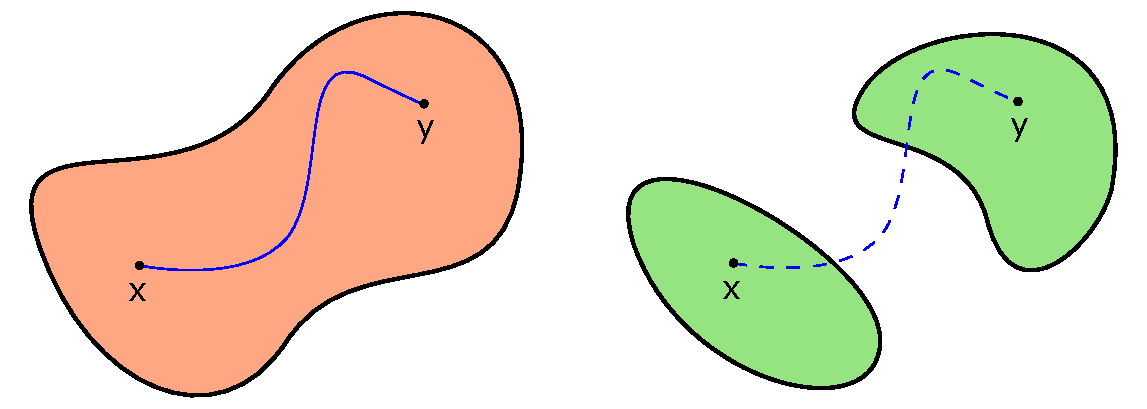
\includegraphics[scale=0.4]{conected-set.pdf}
\end{center}
Множество, изображенное на рисунке слева, является связным, а множество, изображенное справа, не является связным (состоит из двух частей).
\end{frame}

\begin{frame}{Функция нескольких переменных}
\begin{block}{Определение. Функция нескольких переменных}
{\bf Числовой функцией нескольких переменных} называют отображение $f:\ E\to \mathbb{R}$, где $E\subset\mathbb{R}^n$~--- некоторое множество, называемое {\bf множеством определения} функции. Значение функции $f$ в точке $x\in E$ записывают, как $f(x) = f(x_1,\ldots, x_n)$, при этом $x_j$ называют независимыми переменными, а $z=f(x)$ --- зависимой переменной, так как ее значение определяется выбором точки $x$.
\end{block}
\begin{center}
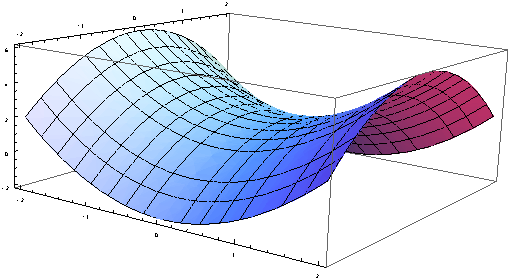
\includegraphics[scale=0.8]{Plot3D.pdf}
\end{center}
При рассмотрении функций двух переменных $z=f(x,y)$ можно рассматривать график функции как поверхность $\Gamma$ в трехмерном пространстве $\mathbb{R}^3$:
$$\Gamma = \{(x,y,z)\mid z=f(x,y),\ (x,y)\in E\}.$$
\end{frame}

\begin{frame}{Линии уровни}
Другой способ визуально представить функцию двух независимых переменных --- это рассмотреть семейство кривых на плоскости, вдоль которых функция является постоянной
$$f(x,y) = const$$
Данные кривые называют {\bf линиями уровня} для функции $f$.
\begin{center}
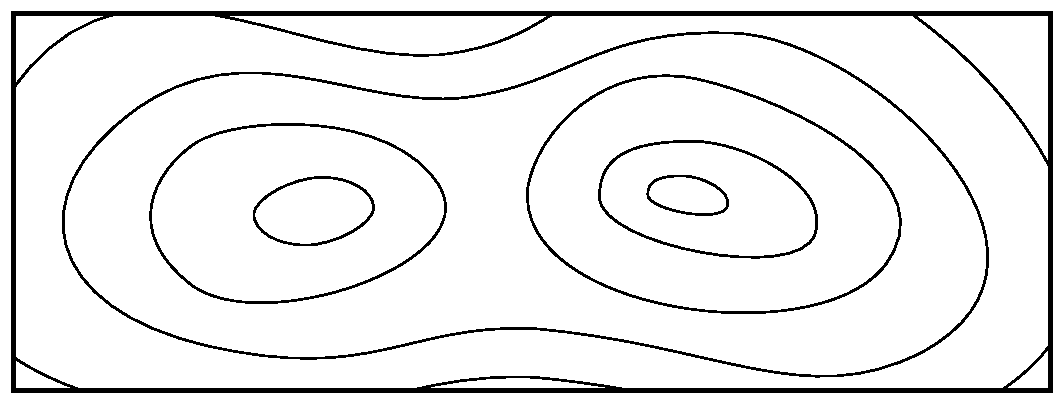
\includegraphics[scale=0.5]{cp.pdf}
\end{center}
\end{frame}

\begin{frame}{Предел функции}
\begin{block}{ Определение. Предел функции}
Пусть функция $f$ определена в некоторой проколотой окрестности точки $a\in\mathbb{R}^n$. Говорят, что число $f_0$ является {\bf пределом} $f(x)$ при $x\to a$, если
$$\forall \varepsilon>0\ \exists \delta>0:\quad |f(x) - f_0|<\varepsilon,\ \forall x\in \dot O_\delta(a).$$
В этом случае пишут $\displaystyle \lim_{x\to a}f(x) = f_0$. 

В случае двух переменных иногда пишут
$$\lim_{x\to x_0,\ y\to y_0} f(x,y) = f_0,$$
а соответствующий предел называют двойным.
\vskip0.5em
Как и в одномерном случае, можно определить сходимость в терминах последовательностей (по Гейне).
\vskip0.5em
Предел $f(x)$ равен $f_0$ при $x\to a$ тогда и только тогда, когда для любой сходящейся к $a$ последовательности точек $\{x^{(k)}\}$ из проколотой окрестности точки $a$ последовательность значений функции в этих точках $f(x^{(k)})$ сходится к $f_0$:
$$\forall \{x^{(k)}\}:\ x^{(k)}\to a,\ x^{(k)}\ne a\ \Rightarrow \ f(x^{(k)})\to f_0.$$
По аналогии с одномерным случаем определяются и бесконечные пределы функций.
\end{block}
\end{frame}

\begin{frame}{Предел функции}
Пусть функция $f$ определена на множестве $M$ и точка $a$ является предельной точкой множества  $M$. Тогда уместно говорить о стремлении $x\to a$ при условии $x\in M$, $x\ne a$.
\begin{block}{ Определение. Предел функции по множеству}
Говорят, что число $f_0$ является пределом функции $f(x)$ при $x\to a$ по множеству $M$ ($x\to a,\ x\in M$), если
$$\forall \varepsilon>0\ \exists \delta>0:\quad |f(x) - f_0|<\varepsilon,\ \forall x\in \dot O_\delta(a)\cap M.$$
В этом случае пишут $\displaystyle \lim_{x\to a,\ x\in M}f(x) = f_0$. 
\end{block}
Частным случаем предела по множеству служат односторонние пределы функции одной переменной.
\end{frame}

\begin{frame}{Непрерывность функции}
\begin{block}{Определение непрерывности в точке}
Говорят, что функция $f(x)$, определенная в некоторой окрестности точки $A\in\mathbb{R}^n$, {\bf непрерывна в точке} $x=A$, если
$$\exists\ \lim_{x\to A}f(x) = f(A).$$
\end{block}
\vskip-0.5em
\pause
Предположим, что функция определена на множестве $M$ и точка $A\in M$ является предельной точкой этого множества. Если точка $A$ не является внутренней для множества~$M$, а принадлежит его границе, то рассматривают следующие определение непрерывности:
\pause
\begin{block}{Определение непрерывности по множеству}
Говорят, что функция $f(x)$, определенная на множестве $M\subset\mathbb{R}^n$, {\bf непрерывна по множеству} $M$ в точке $x=A$, если
$$\exists\ \lim_{x\to A,\ x\in M}f(x) = f(A).$$
Функция считается по определению непрерывной в изолированных точках множества $M$.
\end{block}
\end{frame}

\begin{frame}{Непрерывность функции}
\begin{block}{Определение непрерывности по множеству}
Говорят, что функция $f(x)$, определенная на множестве $M\subset\mathbb{R}^n$, {\bf непрерывна} на множестве $M$, если она непрерывна в каждой точке множества  $M$.
\end{block}
\pause
Свойства непрерывных функций нескольких переменных во многом совпадают со свойствами непрерывных функций одной переменной.
\begin{block}{Свойства непрерывных функций}
\begin{enumerate}
\item Сумма и произведение непрерывных функций непрерывны. Частное непрерывных функций заведомо непрерывно, если делитель (знаменатель) не обращается в ноль.
\item Композиция непрерывных функций непрерывна.
\item Элементарные функции непрерывны на своем множестве определения.
\end{enumerate}
\end{block}
\pause
\begin{block}{Теорема Вейерштрасса}
Пусть функция $f(x)$ непрерывна на компакте $K\subset\mathbb{R}^n$. Тогда она ограничена на множестве~$K$ и достигает на нем своей верхней и нижней грани:
$$\exists x_{min}\in K:\quad f(x_{min}) = \inf_{x\in K}f(x),$$
$$\exists x_{max}\in K:\quad f(x_{max}) = \sup_{x\in K}f(x).$$
\end{block}
\end{frame}


\begin{frame}{Частные производные. Определение}
Рассмотрим функцию $f(x) = f(x_1,\ldots,x_n)$, заданную в окрестности точки $x^0=(x^0_1,\ldots,x^0_n)\in\mathbb{R}^n$. Тогда можно рассмотреть функцию одной переменной $x_k$, фиксировав остальные переменные:
$$\phi(x_k)=f(x^0_1,\ldots, x_{k-1}^0, x_k,x_{k+1}^0,\ldots,x^0_n).$$
Для определения скорости изменения значения функции $f(x)$ при изменении только одной переменной $x_k$ можно рассмотреть производную функции $\phi(x_k)$. Эту производную называют {\bf частной производной} функции $f$ по переменной $x_k$ в точке $x^0$ и обозначают:
$$ \frac{\partial f(x)}{\partial x_k}\Big|_{x=x^0} = \frac{\partial}{\partial x_k}\Big|_{x=x^0}f(x) = \frac{\partial f(x_0)}{\partial x_k}=\frac{\partial f}{\partial x_k}(x^0) = f'_{x_k}(x^0)=f_{x_k}(x^0) = \partial_k f(x_0).$$
\vskip-0.5em
\begin{block}{Определение}
Говорят, что функция $f$, определенная в окрестности точки $x^0\in\mathbb{R}^n$, имеет {\bf частную производную}  по переменной $x_k$ в точке $x^0$, если существует предел
$$\lim_{h\to 0}\frac{f(x^0_1,\ldots, x_{k-1}^0, x^0_k+h,x_{k+1}^0,\ldots,x^0_n) - f(x^0)}{h} = \frac{\partial f(x)}{\partial x_k}\Big|_{x=x^0}.$$
\end{block}
\end{frame}

\begin{frame}{Частные производные. Пример}
\begin{block}{Пример}
Вычислим частные производные функции трех переменных
$$u = x^2+2xy+\cos(x z).$$
Тогда
$$\begin{array}{l}
\frac{\partial u}{\partial x} = 2x+2y-\sin(xz)\, z;\\[0.8em]
\frac{\partial u}{\partial y} = 2x;\\[0.8em]
\frac{\partial u}{\partial z} = -x\sin(x z).
\end{array}$$
В данном случае вычисления производились в произвольной точке $(x,y,z)\in\mathbb{R}^3$. Тогда при дифференцировании по одной из переменных все остальные переменные можно считать постоянными.
\end{block}
\end{frame}

\begin{frame}{Производная по направлению}
Частная производная отражает изменение функции при изменении только одной переменной. Иногда удобно рассматривать производные и по другим направлениям не связанным с координатными осями.

\begin{block}{Определение}
Говорят, что функция $f(x)$, определенная в некоторой окрестности точки $x_0\in\mathbb{R}^n$, имеет в точке $x_0$ {\bf производную по направлению} $l$:
$$l = (l_1,\ldots, l_n),\qquad l_1^2+\cdots+l_n^2 = 1,$$
если существует предел:
$$\frac{\partial f}{\partial l}(x_0) = \lim_{h\to0}\frac{f(x_0+h l) - f(x_0)}{h}.$$
\end{block}
Например, в двумерном случае направление $l$ можно представить в виде:
$$l = (\cos\alpha, \sin\alpha).$$
Тогда производная по направлению $l$ функции $f(x,y)$ примет вид:
$$\frac{\partial f}{\partial l} = \lim_{h\to0}\frac{f(x+h\cos\alpha, y+h\sin\alpha) - f(x,y)}{h}.$$

\end{frame}

\begin{frame}{Дифференцируемость}
\begin{block}{Определение. Дифференцируемая функция}
Говорят, что функция $f$, определенная в окрестности точки $x^0\in\mathbb{R}^n$, {\bf дифференцируема} в точке $x^0$, если для любого достаточно маленького приращения $\Delta x$ переменной $x$:
$$\Delta x = \left( \Delta x_1,\ldots,\Delta x_n\right),$$
приращение значения функции представимо в виде:
$$\Delta f(x^0) = f(x^0+\Delta x) - f(x^0) = \sum_{k=1}^n A_k\, \Delta x_k + o\left(\|\Delta x\|\right),$$
где $A_k$ --- постоянные.
\vskip1em
Линейную часть приращения функции называют {\bf дифференциалом} и обозначают:
$$df\!\left(x^0\right)(\Delta x) = \sum_{k=1}^n A_k\, \Delta x_k.$$
Дифференциал является линейной формой порядка $n$, как функция от $\Delta x$, а также неявно зависит от выбора точки $x^0$.
\end{block}
\end{frame}

\begin{frame}{Дифференцируемость}
\begin{block}{Теорема. Необходимое условие дифференцируемости}
Пусть функция $f$ дифференцируема в точке $x^0\in\mathbb{R}^n$ и 
$$df\!\left(x^0\right)(\Delta x)  = \sum_{k=1}^n A_k\, \Delta x_k.$$
Тогда у функции $f$ существуют частные производные по всем переменным $x_k$ в точке $x^0$ и
$$A_k = \frac{\partial f}{\partial x_k}\!\left(x^0\right).$$
\end{block}
Таким образом, для дифференцируемости функции $f$ необходимо наличие у нее всех частных производных в заданной точке. 
\end{frame}

\begin{frame}{Дифференцируемость}
В одномерном случае существования производной было вполне достаточно для дифференцируемости функции, но в многомерном случае это уже не так.
\begin{block}{Упражнения}
\begin{itemize}
\item Проведите доказательство теоремы о необходимом условии дифференцируемости, аналогично доказательству в одномерном случае.
\item Докажите, что дифференцируемая функция непрерывна.
\item Покажите, что функция
$$f(x,y) = \frac{xy}{x^2+y^2},\quad f(0,0) = 0,$$
не является дифференцируемой, но имеет частные производные в точке $(0,0)$. Покажите, что эта функция не является даже непрерывной.
\end{itemize}
\end{block}
\end{frame}

\begin{frame}{Дифференцируемость}
Вычислим дифференциал функции 
$$u(x_1,\ldots,x_n) = x_k.$$
Тогда
$$u(x+\Delta x) - u(x) = \left(x_k+\Delta x_k\right) - x_k = \Delta x_k.$$
Следовательно, дифференциал имеет вид
$$du(x)(\Delta x) = dx_k(\Delta x) = \Delta x_k.$$
Таким образом, общую формулу для дифференциала функции $f$ можно переписать в виде:
$$df(x^0) = \sum_{k=1}^n \frac{\partial f}{\partial x_k}\!\left(x^0\right)\, dx_k.$$
\begin{block}{Упражнение}
Проверьте, что
$$d\left(\sqrt{x^2+y^2}\right) = \frac{xdx+ydy}{\sqrt{x^2+y^2}}.$$
\end{block}
\end{frame}

\begin{frame}{Дифференцируемость. Достаточное условие}
\begin{block}{Теорема. Достаточное условие дифференцируемости}
Пусть все частные производные $\displaystyle \frac{\partial f}{\partial x_k}$ функции $f(x)$ определены в окрестности точки $x_0$ и непрерывны в точке $x^0$. Тогда функция $f$ является дифференцируемой в точке $x_0$.
\end{block}
\vskip-0.5em
\begin{block}{Доказательство}
Проведем доказательство для $n=2$. Пусть $f = f(x,y)$. Тогда, применяя формулу конечных приращений, получаем:
\begin{multline*}
\Delta f = f(x,y) - f(x_0,y_0) = f(x,y) - f(x,y_0) + f(x,y_0) - f(x_0,y_0) =\\=
\frac{\partial f}{\partial y}(x,\eta)(y-y_0) +\frac{\partial f}{\partial x}(\xi,y_0)(x-x_0).
\end{multline*}
Из непрерывности частных производных следует, что
$$\frac{\partial f}{\partial y}(x,\eta) = \frac{\partial f}{\partial y}(x_0,y_0)+o(1),\qquad \frac{\partial f}{\partial x}(\xi,y_0) = \frac{\partial f}{\partial x}(x_0,y_0)+o(1).$$
Таким образом,
$$\Delta f = \frac{\partial f}{\partial x}(x_0,y_0)\Delta x+\frac{\partial f}{\partial y}(x_0,y_0)\Delta y + o\left(|x-x_0|\right)+o\left(|y-y_0|\right).$$
%Из неравенства
%$$|x-x_0|+|y-y_0|\le 2\sqrt{(x-x_0)^2+(y-y_0)^2}.$$
%следовательно
%$$o\left(|x-x_0|\right)+o\left(|y-y_0|\right) =o\left(|x-x_0|+|y-y_0|\right) = o\left(\sqrt{(x-x_0)^2+(y-y_0)^2}\right).$$
\end{block}
\end{frame}

\begin{frame}{Частные производные. Градиент}
\begin{block}{Определение. Градиент}
Если функция $f(x)$, $x\in\mathbb{R}^n$, имеет частные производные по всем переменным ($n$ штук) в фиксированной точке $x^0$, то числовой вектор
$$\grad f\, \Big|_{x=x^0} = \left(\frac{\partial f}{\partial x_1}\left(x^0\right),\ldots, \frac{\partial f}{\partial x_n}\left(x^0\right)\right)$$
называют {\bf градиентом} функции $f$ в точке $x^0$. То есть градиент --- это вектор, составленный из частных производных функции $f$ в точке $x^0$. 
\end{block}

\begin{block}{Определение. Производные высших порядков}
Если частная производная функции $f(x)$ по переменной $x_k$ определена в некоторой окрестности точки $x^0\in\mathbb{R}^n$, то можно определить {\bf частные производные второго порядка}:
$$\frac{\partial^2 f}{\partial x_k\partial x_m}\left( x^0 \right) = \frac{\partial}{\partial x_m}\Big|_{x = x^0} \frac{\partial f(x)}{\partial x_k},\quad k=1,\ldots, n,$$
как частные производные по переменной $x_m$ от функции $\displaystyle \frac{\partial f(x)}{\partial x_k}$. Аналогично определяются производные третьего порядка и далее.
\end{block}
\end{frame}

\begin{frame}{Частные производные. Пример}
\begin{block}{Пример}
Пусть
$$f = x^2+2xy.$$
Тогда
$$\begin{array}{ll}
\frac{\partial f}{\partial x} = 2x+2y;&
\frac{\partial f}{\partial y} = 2x;\\[0.8em]
\frac{\partial^2 f}{\partial x^2} = \frac{\partial}{\partial x}\left( 2x+2y\right)  =2;&
\frac{\partial^2 f}{\partial x \partial y} = \frac{\partial}{\partial y}\left( 2x+2y\right)  =2;\\[0.8em]
\frac{\partial^2 f}{\partial y \partial x} = \frac{\partial}{\partial x}\left( 2x \right)  =2;&
\frac{\partial^2 f}{\partial y^2} = \frac{\partial}{\partial y}\left(2x\right)  = 0.
\end{array}$$
Таким образом, для функции двух переменных существует четыре частных производных второго порядка. Они образуют матрицу $2\times2$. В общем случае размерности $n$ мы получим квадратную матрицу размера $n\times n$.
\end{block}
\end{frame}

\begin{frame}{Свойства градиента}
\begin{block}{Предложение}
Пусть функция $f$ дифференцируема в точке $x$. Тогда для производной по направлению $l$ справедлива формула:
$$\frac{\partial f}{\partial l}(x) = \sum_{k=1}^n l_k\cdot \frac{\partial f}{\partial x_k} = \left( l_1 \frac{\partial}{\partial x_1} + \cdots + l_n \frac{\partial}{\partial x_n} \right) f(x) = \langle l,\, \grad f \rangle.$$
То есть производная по направлению $l$ совпадает с проекцией вектора $\grad f$ на вектор $l$.
\end{block}
\begin{block}{Доказательство}
Функция $f$ является дифференцируемой:
$$f(x+\Delta x) - f(x) =  \sum_{k=1}^n \frac{\partial f}{\partial x_k} \Delta x_k + o\left(\|\Delta x\|\right).
$$
Пусть $\Delta x = h l$. Тогда $\displaystyle\quad \|\Delta x\| = |h|\,\|l\| = |h|,\quad \Delta x_k  = l_k h.$

Следовательно,
$$\pp{f}{l} = \lim_{h\to0}\frac{f(x+h l) - f(x)}{h} = \lim_{h\to 0}\frac{1}{h}\left( \sum_{k=1}^n \frac{\partial f}{\partial x_k} l_k h + o(h)\right) = \sum_{k=1}^n \frac{\partial f}{\partial x_k} l_k.$$

\end{block}
\end{frame}

\begin{frame}{Геометрический смысл градиента}
Производная по направлению $l$ характеризует скорость роста функции в этом направлении. Мы видим, что производная по направлению совпадает с проекцией направляющего вектора $l$ на вектор градиента $\grad f$. Следовательно, направление, в котором функция растет сильнее всего, совпадает с направлением градиента.
\vskip1em
Направление градиента --- это направление наискорейшего роста функции, а модуль градиента --- это скорость роста функции в этом направлении.

\begin{center}
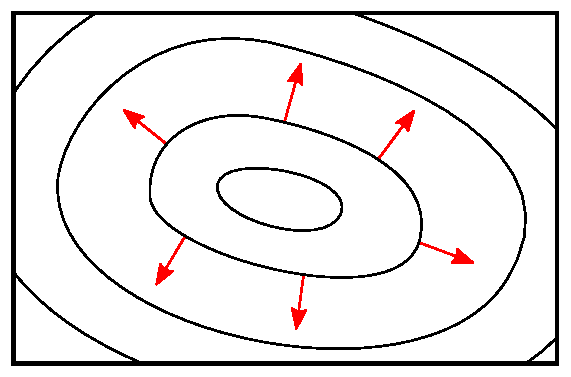
\includegraphics[scale=0.5]{grad.pdf}
\end{center}
Если рассмотреть линии уровни функции, то есть кривые на которых функция постоянна, то градиент будет ортогонален линиям уровня. {\bf Докажите это} в двумерном случае.
\end{frame}

\begin{frame}{Правила дифференцирования}
Поскольку частные производные --- это производные от функции многих переменных, как от функции одной переменной при фиксации остальных переменных, то все правила дифференцирования сохраняют силу. Остановимся только на дифференцировании сложной функции.

\begin{block}{Правило дифференцирования сложной функции}
Пусть функция $f(x) = f(x_1,\ldots,x_n)$ дифференцируема в точке $x^0\in\mathbb{R}^n$, $n$ функций $g_j(t) = g_j(t_1,\ldots,t_m)$ дифференцируемы в точке $t^0\in\mathbb{R}^m$, и $g_j(t^0) = x^0_j$, где $j=1,\ldots,n$.  Тогда сложная функция $F(t) = f(g(t))$ дифференцируема в точке $t^0$ и справедливы формулы
$$\pp{F}{t_k} = \pp{}{t_k}\Big|_{t=t^0}\, f(g_1(t),\ldots,g_n(t)) = \sum_{s=1}^n \pp{f}{x_s}(g_1(t^0),\ldots,g_n(t^0))\, \pp{g_s}{t_k}(t^0).$$
\end{block}
\end{frame}

\begin{frame}{Правила дифференцирования}
\begin{block}{Пример}
Пусть на прямой задана потенциальная энергия $U(x)$. Тогда уравнение Ньютона имеет вид:
$$m\frac{dv}{dt} = - \frac{dU}{dx}.$$
Определим функцию 
$$ E(x,v) = \frac{m v^2}{2} + U(x).$$
Пусть $x(t)$, $v(t) = \dot x(t)$ --- решение уравнений Ньютона. Тогда
$$\frac{d}{dt} E(x(t),v(t)) = \pp{E}{x}\frac{dx}{dt} + \pp{E}{v} \frac{dv}{dt} = U'(x(t))v(t) + m v(t) \left( - \frac{1}{m}U'(x(t))\right) = 0.$$
Таким образом, функция $E(x,v)$ сохраняет свое значение --- это закон сохранения энергии.
\end{block}
\end{frame}

\begin{frame}{Теорема Шварца}
\begin{block}{Теорема о равенстве смешанных производных}
Пусть частные производные $\displaystyle \frac{\partial^2 f}{\partial x\partial y}$ и $\displaystyle \frac{\partial^2 f}{\partial y\partial x}$ функция $f(x,y)$ определены в некоторой окрестности точки $(x_0,y_0)$ и {\bf непрерывны} в этой точке. Тогда они совпадают:
$$ \frac{\partial f^2}{\partial x\partial y}(x_0,y_0) = \frac{\partial f^2}{\partial y\partial x}(x_0,y_0).$$
\end{block}
Теорема естественным образом обобщается на случай функции нескольких переменных и на производные выше второго порядка. Так значение смешанной производной не зависит от порядка дифференцирования, если соответствующие частные производные непрерывны.
\pause
\begin{block}{Замечание}
Условие непрерывности является достаточным, но отнюдь не является необходимым. Смешанные производные могут совпадать и в случае, когда непрерывность не имеет место.
\end{block}
\vskip-0.5em
\begin{block}{Упражнения}
\begin{itemize}
\item Докажите теорему.
\item \vskip-1em Рассмотрите пример
$\quad\displaystyle f(x,\;y)= \left\{ \begin{array}{ll}
\displaystyle \frac{xy(x^2-y^2)}{x^2+y^2},& x^2+y^2>0; \\[0.8em]
0,& x=y=0. \end{array}\right.$
\end{itemize}
\end{block}
\end{frame}

\begin{frame}{Старшие дифференциалы. Формула Тейлора}
Для дифференцируемой функции $f(x)$, $x\in\mathbb{R}^n$, справедлива формула линеаризации:
$$f(x+y) = f(x) + \langle \grad f(x),\, y \rangle +o\left(\|y\|\right).$$
Часто возникает необходимость приближения более высокой точности. 
\begin{block}{Теорема. Формула Тейлора}
Пусть все частные производные функция $f$ до порядка $m$ включительно определены в некоторой окрестности точки $x\in\mathbb{R}^n$ и непрерывны в этой точке. Тогда справедлива формула Тейлора:
\begin{multline*}
f(x+y) = f(x) + \sum_{k=1}^n \pp{f(x)}{x_k}y_k + \frac{1}{2}\sum_{k,r=1}^n 
\frac{\partial^2f(x)}{\partial x_k\partial x_r}y_k y_r+
\cdots
\\+\frac{1}{m!}\sum_{k_1,\ldots,k_m = 1}^n \ \frac{\partial^m f(x)}{\partial x_{k_1}\cdots\partial x_{k_m}}\ y_{k_1}\cdots y_{k_m}+ o\left(\|y\|^{m}\right).
\end{multline*}
\end{block}
\end{frame}

\begin{frame}{Старшие дифференциалы. Формула Тейлора}
\begin{block}{Пример}
Для функции двух переменных получаем:
\begin{multline*}
f(x+\Delta x,y+\Delta y)  = f(x,y) + \pp{f}{x}\,\Delta x+\pp{f}{y}\,\Delta y+\\
\frac{1}{2}\left( \frac{\partial^2 f}{\partial x^2}\,\Delta x^2+2 \frac{\partial^2 f}{\partial x \partial y}\,\Delta x\Delta y+\frac{\partial^2 f}{\partial y^2}\,\Delta y^2\right)+\cdots,
\end{multline*}
где производные взяты в точке $(x,y)$.
\end{block}
{\bf Второй дифференциал} функции $f(x,y)$ определяется как:
$$d^2f(x,y) = d(df(x,y)),$$
Следовательно,
$$d^2f(x,y) = d\left(  \pp{f}{x}\,d x+\pp{f}{y}\,d y\right)  =  \frac{\partial^2 f}{\partial x^2}\,dx^2+2 \frac{\partial^2 f}{\partial x \partial y}\,dx dy+\frac{\partial^2 f}{\partial y^2}\,dy^2.$$
Аналогично определяются дифференциалы старших порядков.

Мы видим, что формулу Тейлора можно записать в виде:
$$f(x+\Delta x,y+\Delta y)  = f(x,y) +df(x,y)(\Delta x,\Delta y) +
\frac{1}{2}d^2f(x,y)(\Delta x,\Delta y)+\cdots
$$
\end{frame}

\begin{frame}{Локальные экстремумы}
\begin{block}{Определение. Локальный экстремум}
Точка $x^0\in\mathbb{R}^n$ называется {\bf точкой локального максимума} (или минимума) функции $f(x)$, определенной в некоторой окрестности этой точки, если существует окрестность $U$ точки $x^0$ такая, что для всех $x\in U$, $x\ne x^0$ справедливо неравенство:
$$f(x) < f(x^0),\quad \text{или}\quad f(x) > f(x^0).$$
Точки локальных минимумов и максимумов называют {\bf точками локального экстремума} функции.
\end{block}
\pause
Пусть функция рассматривается на множестве $M\subset\mathbb{R}^n$, для которого точка $x^0\in M$ не является внутренней, а например, является точкой границы. Тогда данное выше определение дополняют условием $x\in M$.
\begin{block}{Определение. Условный локальный экстремум}
Точка $x^0\in M$ называется {\bf точкой условного локального максимума} (или минимума) функции $f(x)$ при условии $x\in M$, если существует окрестность $U$ точки $x^0$ такая, что для всех $x\in U\cap M$, $x\ne x^0$ справедливо неравенство:
$$f(x) > f(x^0),\quad \text{или}\quad f(x)<f(x^0).$$
\end{block}
Иногда говорят о внутренних и граничных точках локального экстремума.
\end{frame}

\begin{frame}{Достаточное условие экстремума}
В многомерном случае справедлив аналог теоремы Фурье:
\begin{block}{Теорема. Достаточные условия локального экстремума}
Пусть функция $f(x)$ дифференцируема в точке $x^0\in\mathbb{R}^n$ и имеет в этой точке локальный экстремум. Тогда в этой точке градиент функции равен нулю:
$$\grad f(x^0) = 0\quad \iff\quad \pp{f}{x_k}(x^0) = 0,\quad k=1,\ldots,n.$$
\end{block}
Таким образом, во всех точках локального экстремума равны нулю все частные производные. Такие точки принято называть {\bf критическими}.
\begin{block}{Доказательство}
Докажем от противного. Пусть в точке $x^0$ имеет место локальный экстремум, а градиент не обращается в ноль. Можно считать, что $\ \displaystyle \pp{f}{x_1}(x^0)\ne 0$. Тогда функция $g(t) = f(x_1^0+t,x_2^0,\ldots,x_n^0)$ одной переменной $t$, очевидно, дифференцируема и имеет экстремум в точке $t=0$, но
$$g'(0) = \frac{d}{dt}f(x_1^0+t,x_2^0,\ldots,x_n^0) = \pp{f}{x_1}(x^0)\ne0,$$
что противоречит теореме Ферма.
\end{block}
\end{frame}

\begin{frame}{Необходимое условие}
Как и в одномерном случае, для исследования критической точки можно рассмотреть второй дифференциал функции.
\begin{block}{Теорема. Необходимые условия локального экстремума}
Пусть функция $f(x)$ дважды дифференцируема в точке $x^0\in\mathbb{R}^n$, точка $x^0$ является критической $\grad f(x^0)=0$ и второй дифференциал функции $f$ в этой точке является положительно (отрицательно) определенной квадратичной формой. Тогда эта точка является минимумом~(максимумом).
\end{block}

\begin{block}{Двумерный случай}
Для функции двух переменных условие максимума примет вид:
$$d^2 f = \frac{\partial^2 f}{\partial x^2}\,dx^2+2 \frac{\partial^2 f}{\partial x \partial y}\,dx dy+\frac{\partial^2 f}{\partial y^2}\,dy^2<0,$$
для произвольных приращений $dx$ и $dy$, кроме $dx=dy=0$.
\end{block}

Вопрос о знаке квадратичной формы детально изучается в линейной алгебре.
\end{frame}

\begin{frame}{Достаточное условие экстремума}
\begin{block}{Пример}
Рассмотрим функцию $f(x) = x^2+x+2y^2+x y$. Задача стоит в поиске локальных и глобальный точек минимума и максимума. 
\vskip1em
Функция, очевидно, является дифференцируемой. Критические точки определяются из системы уравнений:
$$\left\{ \begin{array}{l}
\displaystyle \pp{f}{x} = 0;\\[1em]
\displaystyle \pp{f}{y} = 0,
\end{array}\right. \quad \iff \quad
\left\{ \begin{array}{l}
\displaystyle 2x+1+y= 0;\\
\displaystyle 4y+x = 0,
\end{array}\right.
\quad \iff \quad
\left\{ \begin{array}{l}
\displaystyle x = -4/7;\\
\displaystyle y = 1/7.
\end{array}\right.$$
Вычислим $d^2 f$ в этой точке:
$$d^2 f = 2dx^2+2dxdy+4dy^2 = dx^2+(dx+dy)^2+3dy^2>0,$$
при $dx$ и $dy$ неравных нулю одновременно. Следовательно, рассматриваемая точка является точкой минимума.
\end{block}
\end{frame}

\begin{frame}{Критерий Сильвестра}
В алгебре доказывается теорема, позволяющая легко проверять знак второго дифференциала.
\begin{block}{Теорема. Критерий Сильвестра}
Пусть $F$ --- квадратичная форма порядка $n$:
$$F(y) = \langle A y, y \rangle = \sum_{i,\, j=1}^n a_{ij}\, y_i y_j,$$
где $A$ --- симметричная матрица $a_{ij} = a_{ji}$. Тогда $F$ положительно определена тогда и только тогда, когда все угловые миноры $A_k$, $k=1,\ldots,n$ положительны, и $F$ отрицательно определена тогда и только тогда, когда знаки $A_k$ чередуются так, что $A_1<0$.
\end{block}
Угловые миноры $A_k$ матрицы $A$ --- это определители:
$$A_1 = a_{11},\quad A_2 = \left| \begin{array}{cc}
a_{11}&a_{12}\\
a_{21}&a_{22}
\end{array}\right|, 
\quad\cdots\quad
A_n = \left|\begin{array}{cccc}
a_{11}&a_{12}&\cdots&a_{1n}\\
a_{21}&a_{22}&\cdots&a_{2n}\\
& & \cdots & \\
a_{n1}&a_{n2}&\cdots&a_{nn}
\end{array}\right|.$$
\end{frame}

\begin{frame}{Условный экстремум}
Предположим, что нам необходимо исследовать функцию $f(x,y)$ на условный экстремум, если условие имеет вид $g(x,y) = 0$. Функции $f$ и $g$ предполагаются непрерывно дифференцируемыми.
\begin{block}{Прямой метод}
Если уравнение кривой $g(x,y)=0$ можно переписать в параметрическом виде $x=x(t)$,~$y=y(t)$, то исследование функции $f$ можно свести к исследованию функции~$F(t) = f(x(t),y(t))$ одной переменной $t$.
\end{block}
\begin{block}{Метод множителей Лагранжа}
Составим функцию Лагранжа:
$$L(x,y,\lambda) = f(x,y) + \lambda g(x,y).$$
\end{block}
\vskip-1em
\begin{block}{Теорема Лагранжа}
Пусть точка $(x_0,y_0)$ --- точка условного экстремума $f$ и $\grad{g}(x_0,y_0)\ne0$. Тогда найдется такая постоянная $\lambda_0$, что точка $(x_0,y_0,\lambda_0)$ будет критической точкой функции $L$, то есть
$$\pp{L}{x}=0,\quad \pp{L}{y}=0,\quad \pp{L}{\lambda} = 0,$$
в точке $(x_0,y_0,\lambda_0)$.
\end{block}
\end{frame}

\begin{frame}{Теоремы о неявной функции}
Предположим, что функция $y = f(x)$, $x\in\mathbb{R}^n$, задана неявно уравнением:
$$F(x_1,\ldots, x_n, y) = 0.$$
Возникает вопрос об условиях разрешимости этого уравнения.

\begin{block}{Теорема о неявной функции}
Пусть $F(x,y)$ имеет непрерывные частные производные в точке $(x^0,y^0)\in\mathbb{R}^{n+1}$, точка $(x^0,y^0)$ удовлетворяет уравнению $F(x^0,y^0)=0$, частная производная $F$ по $y$ не равна нулю:
$$\pp{F}{y}(x^0,y^0)\ne 0.$$
Тогда существует окрестность $U$ точки $x^0$, в которой уравнение $F(x,y)=0$ однозначно определяет непрерывную функцию $y = f(x)$, для которой $y^0=f(x^0)$. Функция $f(x)$ имеет непрерывные в точке $x^0$ частные производные.
\end{block}
\begin{block}{Следствие}
Дифференцируя равенство $F(x,f(x))=0$ по переменной $x_k$, получаем формулу для частных производных функции $f(x)$:
$$\pp{F}{x_k}+ \pp{F}{y}\, \pp{f}{x_k}= 0
\quad\Rightarrow\quad
\pp{f}{x_k}(x^0) = - \pp{F}{x_k}(x^0,y^0)\left( \pp{F}{y}(x^0, y^0) \right)^{-1}.$$
\end{block}
\end{frame}

\begin{frame}{Замены координат}
Рассмотрим $n$ отображений $y_1 = f_1(x),\ldots, y_n = f_n(x)$, где $x\in\mathbb{R}^n$. Тогда вектор $f(x) = (f_1(x),\ldots,f_n(x))$ можно также интерпретировать, как точку $n$-мерного пространства. Говорят, что $f$ задает отображение из $\mathbb{R}^n$ в $\mathbb{R}^n$. Говорят, что отображение $y=f(x)$ непрерывно (или дифференцируемо), если таковыми являются все функции $f_i(x)$.
\begin{block}{Определение}
Матрицей Якоби дифференцируемого отображения $f$ называют матрицу:
$$\mathcal{J}(x) = \pp{f}{x} =  \left(\begin{array}{cccc}
\pp{f_1}{x_1}&\cdots&\pp{f_1}{x_n}\\
& \cdots & \\
\pp{f_n}{x_1}&\cdots&\pp{f_n}{x_n}
\end{array}\right).$$
Якобианом отображения $f$ называют определитель этой матрицы  $J(x) = \det \mathcal{J}(x)$.
\end{block}
\begin{block}{Определение}
Отображение $f:\ \mathbb{R}^n\to\mathbb{R}^n$ является регулярным (невырожденным) в точке $x^0$, если оно непрерывно дифференцируемо в окрестности точки $x^0$ и якобиан отображения не обращается в ноль: $J(x^0)\ne0$.
\end{block}
\end{frame}

\begin{frame}{Обратное отображение}
Рассмотрим вопрос о том, когда отображение $y=f(x)$ является обратимым.
\begin{block}{Теорема об обратном отображение}
Пусть отображение $y = f(x)$ регулярно в точке $x_0\in\mathbb{R}^n$. Тогда существует окрестность $U$ точки $x^0$ такая, что уравнение $y=f(x)$ однозначно разрешимо относительно $x$, и соответствующее отображение $x = g(y)$ регулярно в $U$.
\end{block}
\begin{block}{Следствие}
Вычислим частные производные $\pp{g_k}{y_m}(y)$, продифференцировав равенство:
$$y_m = f_m(g(y))
\quad \Rightarrow \quad 
 \sum_{j=1}^n \pp{f_m}{x_j}\pp{g_j}{y_s} = \delta_{s,m} =  \left\{
 \begin{array}{ll}
1,& s=m;\\
0,& s\ne m.
\end{array}\right.
$$
Таким образом, матрицы Якоби взаимно обратных отображений $\pp{g}{y}$ и $\pp{f}{x}$ являются взаимно обратными матрицами. Как известно из алгебры, обратная матрица существует тогда и только тогда, когда определитель матрицы не равен нулю. В этом и заключается условие регулярности отображений. 
\end{block}
\end{frame}

\begin{frame}{Примеры замен}
Некоторые замены переменных крайне часто используются на практике.
\begin{block}{Полярные координаты}
Переход к полярным координатам на плоскости имеет вид:
$$\begin{array}{l}
x = r \cos(\phi);\\
y = r \sin(\phi),
\end{array}
\quad\iff\quad
\begin{array}{l}
r = \sqrt{x^2+y^2};\\
\phi =\arctg\frac{y}{x}.
\end{array}
$$
Найдем матрицу Якоби:
$$\mathcal{J} = \pp{(x,y)}{(r,\phi)} = \left(\begin{array}{cc}
\cos(\phi)& -r\sin(\phi)\\
\sin(\phi)& r\cos(\phi)
\end{array}\right).$$
Следовательно, Якобиан перехода от $(r,\phi)$ к $(x,y)$ равен
$$J(r,\phi) = r \cos^2(\phi)+r\sin^2(\phi) = r.$$
Замена координат не является регулярной при $r=0$ или $x=y=0$. Действительно, в этих точках отображение даже не является взаимно однозначным.
\end{block}
\end{frame}

\begin{frame}{Примеры замен}
\begin{block}{Упражнения}
Найдите Якобианы перехода к сферическим координатам:
$$\begin{array}{l}
x = r \cos(\phi)\sin(\theta);\\
y = r \sin(\phi)\sin(\theta);\\
z = r \cos(\theta),
\end{array}
$$
и цилиндрическим координатам:
$$\begin{array}{l}
x = r \cos(\phi);\\
y = r \sin(\phi);\\
z = z,
\end{array}
$$
Определите, где отображения являются обратимыми.
\end{block}
\end{frame}

\begin{frame}{Формула линеаризации}
Пусть $y = f(x)$ --- регулярное отображение в окрестности точки $x^0$. Построим линейное приближение для $f(x)$ в случае, когда $x$ близко к $x^0$. Для каждой функции $f_m(x)$ имеем:
$$f_m(x) = f_m(x^0) + \sum_{k=0}^n \pp{f_m}{x_k}(x^0)\,(x_k-x_k^0) + o(\|x-x^0\|).$$
Следовательно, в матричной записи получаем, что
$$f(x) = f(x^0) + \pp{f}{x}(x^0)\, (x-x^0)+o(\|x - x^0\|),$$
где $\ds \pp{f}{x}$ --- матрица Якоби размера $n\times n$. 
\vskip1em
Таким образом, линейным приближением для отображения $f$ в окрестности точки $x^0$ является линейный оператор с матрицей Якоби в базисе с координатами $(x_1,\ldots,x_n)$.
\vskip1em
Следовательно, если отображение $f$ регулярно в точке $x^0$ (то есть определитель матрицы Якоби не равен нулю), то набор векторов $v_k=\grad f_k(x^0)$ является линейно независимым.
\end{frame}

\begin{frame}{Якобиан отображения и ориентируемый объем}
\begin{block}{Определение}
Рассмотрим $n$-мерный параллелепипед с вершинами в точках $A^1,\ldots,A^n$. Тогда его {\bf ориентируемый объем} определяется как
$$Vol(A) =\det(A),$$
где матрица $A$ составлена из вектор-столбцов $A^k$. 
\vskip1em
Ориентируемый объем может быть как положительным, так и отрицательным в зависимости от взаимного расположения точек $A^k$. Объемом параллелепипеда называют величину $|Vol(A)|$.
\end{block}
\end{frame}

\begin{frame}{Якобиан отображения и ориентируемый объем}
Пусть $y = f(x)$ --- регулярное в точке $x^0$ отображение, а $\Delta x$ --- малое приращение аргумента~$x$. Учитывая формулу линеаризации, можно считать, что образом прямоугольного параллелепипеда $D$ со сторонами $\Delta x_1,\ldots,\Delta x_n$ является параллелепипед $M$ с вершинами 
$$u_1=f(x^0+\Delta x_1,x_2,\ldots,x_n)-f(x^0) \approx \pp{f}{x_1}\Delta x_1,$$
$$\ldots$$
$$ u_n = f(x^0,x_2,\ldots,x_n+\Delta x_n)-f(x^0) \approx \pp{f}{x_n}\Delta x_n.$$
Следовательно, объем параллелепипеда $M$ связан с объемом параллелепипеда $D$ по формуле
$$Vol(M) = \det\mathcal{J}(x^0)\, \Delta x_1\cdots\Delta x_n = J(x^0)\, Vol(D).$$
Таким образом якобиан отображения является коэффициентом преобразования ориентированного объема элемента пространства при отображении $f$ в точке $x^0$.
\end{frame}

\begin{frame}{Площадь плоской области}
Определим понятие площади для плоского ограниченного множества $M\subset\mathbb{R}^2$.
\begin{block}{Определение. Клеточное множество}
Если $M$ представляется в виде объединения конечного числа прямоугольников, пересекающихся лишь по границам, то $M$ называют {\bf клеточным} множеством. 
\end{block}
Тогда площадь $S_M$ клеточного множества $M$ --- это сумма площадей соответствующих прямоугольников. 
\begin{block}{Определение. Площадь}
Будем говорить, что множество $D\subset\mathbb{R}^2$ имеет {\bf площадь} $S(D) = S_D$, если для любого $\varepsilon>0$ найдутся два клеточных множества $\Omega$ и $\omega$ такие, что 
$$\omega\subset D \subset \Omega,\quad S_\omega<S_D<S_\Omega,\quad S_\Omega-S_\omega<\varepsilon.$$
Множества, имеющие площадь, называют {\bf измеримыми} (по Жордану).
\end{block}
\begin{block}{Замечание}
Область, ограниченная гладкой кривой, всегда измерима. Не все множества на плоскости вообще имеют какую-либо площадь.
\end{block}
Аналогично определяются понятия измеримости и объема множества в трехмерном пространстве $\mathbb{R}^3$, и в случае большей размерности.
\end{frame}

\begin{frame}{Двойной интеграл}
Предположим, что $f(x,y)$ --- скалярная функция, заданная на ограниченном множестве $D\subset\mathbb{R}^2$. Определим объем тела в трехмерном пространстве, которое лежит между графиком функции $z=f(x,y)$ и плоскостью $xOy$, при $(x,y)\in D$.
\vskip1em
Предположим, что $D$ --- измеримое множество. Разобьем $D$ на конечное число измеримых частей $D_1,\ldots, D_m$:
$$D = \bigcup_{k=1}^m D_k,\qquad D_i\cap D_j = \emptyset,\ i\ne j.$$
В каждом множестве $D_k$ выберем опорную точку $A_k = (x_k,y_k)\in D_k$.
\vskip1em
 Диаметром $d_k = d(D_k) $ множества $D_k$ называют расстояние между максимально удаленными точками множества $D_k$:
 $$d(D_k) = \sup_{a,b\in D_k}\|a - b\|.$$
 Параметром разбиения будем называть величину $d = \max d_k$.
 \vskip1em
 Интегральной суммой будем называть величину:
 $$\sum_{k=1}^m f(A_k)\, S(D_k).$$
\end{frame}

\begin{frame}{Двойной интеграл. Определение}
\begin{block}{Определение}
Будем говорить, что функция $f(x,y)$, определенная на измеримом множестве $D$, интегрируема в $D$, если  существует предел интегральных сумм:
$$\iint\limits_D f(x,y)dxdy = \lim_{d\to 0}\, \sum_{k=1}^m f(A_k)\, S(D_k),$$
при стремлении параметра разбиения к нулю, для произвольного выбора разбиения и опорных точек.
\end{block}
Аналогичным образом определяется тройной интеграл по трехмерному измеримому множеству:
$$\iiint\limits_D f(x,y,z)dxdydz.$$
В многомерном случае пишут просто
$$\int\limits_D f(x_1,\ldots,x_n)dx_1\cdots dx_n = \int\limits_D f(x) dx,$$
где $D$ --- ограниченное измеримое множество в $\mathbb{R}^n$.
\end{frame}

\begin{frame}{Двойной интеграл. Свойства}
\begin{block}{Свойства}
\begin{enumerate}
\item Если функция $f(x)$ непрерывна на замыкании $\overline{D}$ измеримого множества $D\in\mathbb{R}^n$, то она интегрируема.
\item Площадь (объем) измеримого множества $D\subset\mathbb{R}^n$ можно вычислить как
$$S(D) = \int_D 1dx.$$
\item Линейность:
$$\int_D \left( f(x)+g(x)\right) \, dx = \int_D f(x)dx+\int_D g(x)dx,\qquad \int_D A\, f(x)\,dx = A\int_D f(x)\,dx. $$
\item Аддитивность. Пусть $D_1$ и $D_2$ --- два непересекающихся ($D_1\cap D_2 = \emptyset$) измеримых множества в $\mathbb{R}^n$, и функция $f$ интегрируема на $D_1$ и $D_2$. Тогда $f$ интегрируема на измеримом множестве $D_1\cup D_2$ и 
$$\int_{D_1\cup D_2}f(x)\,dx = \int_{D_1} f(x)\,dx+\int_{D_2}f(x)\,dx.$$
\end{enumerate}
\end{block}
\end{frame}

\begin{frame}{Двойной интеграл. Свойства}
\begin{block}{Интегрирование неравенств}
Пусть $f(x)$ и $g(x)$ --- интегрируемые функции на измеримом множестве $D\subset\mathbb{R}^n$. Если справедливо неравенство
$$f(x)\le g(x),\qquad \forall x\in D,$$
то
$$\int_D f(x)dx \le \int_D g(x)dx.$$
\end{block}
\vskip-0.5em
\begin{block}{Теорема о среднем}
Пусть $f(x)$ --- непрерывная на связном измеримом компакте $D\subset\mathbb{R}^n$ функция. Тогда найдется такая точка $\xi\in D$, что
$$\int_D f(x)dx = f(\xi) \int_D 1\, dx = f(\xi) S(D).$$
\end{block}
\vskip-0.5em
\begin{block}{Оценка интеграла}
Если функция $f(x)$ интегрируема на измеримом множестве $D\subset\mathbb{R}^n$, то функция $|f(x)|$ также интегрируема и 
$$\left| \int_D f(x)dx \right| \le \int_D |f(x)| \, dx.$$
\end{block}
\end{frame}

\begin{frame}{Двойной интеграл. Сведение к повторному}
\begin{block}{Теорема}
Пусть $f(x,y)$ непрерывна в прямоугольнике 
$$\Pi =[a,b]\times[c,d] =\left\{ (x,y)\in\mathbb{R}^2 \mid
 x\in[a,b],\ y\in[b,c] \right\}.$$
Тогда
$$\iint_\Pi f(x,y)dxdy = \int_a^b\left( \int_c^d f(x,y)dy \right) dx = \int_c^d\left( \int_a^b f(x,y)dx \right) dy.$$
\end{block}
Интегралы в правой части последнего равенства принято называть повторными, поскольку интегрирование сначала производится только по одной переменной, и только затем --- по второй. Часто их записывают в виде
$$\int_a^b dx \int_c^d f(x,y)dy,\quad \int_c^d dy \int_a^b f(x,y)dx,$$
соответственно.
\begin{block}{Следствие}
Если функция $f$ представляется в виде $f(x,y) = \phi(x)\psi(y)$, то
$$\iint_\Pi f(x,y)dxdy =  \left( \int_a^b \phi(x) dx \right) \cdot \left( \int_c^d \psi(y) dy \right).$$
\end{block}
\end{frame}

\begin{frame}{Двойной интеграл. Сведение к повторному}
\begin{block}{Теорема}
Пусть $y_1(x)\le y_2(x)$ --- пара непрерывных на $[a,b]$ функций, функция $f(x,y)$ непрерывна на множестве
$$Q =\left\{ (x,y)\in\mathbb{R}^2 \mid
 x\in[a,b],\ y_1(x)\le y\le y_2(x) \right\}.$$
Тогда
$$\iint_Q f(x,y)dxdy =\int_a^b dx \int_{y_1(x)}^{y_2(x)}f(x,y)dy.$$
\end{block}
\begin{center}
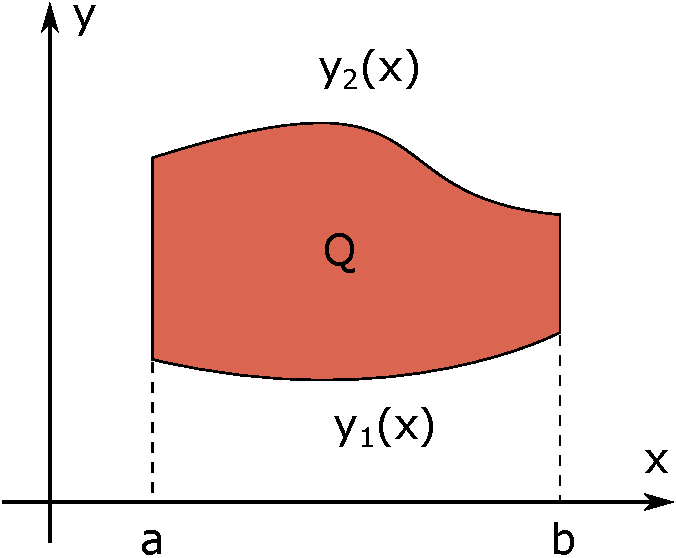
\includegraphics[scale=0.4]{iintQ.pdf}
\end{center}
\end{frame}

\begin{frame}{Двойной интеграл. Замена переменных}
Другой способ вычисления двойного интеграла связан с введением новых координат.
\begin{block}{Теорема}
Пусть $f(x)$ --- непрерывная функция на измеримом компакте $D\subset\mathbb{R}^n$ с кусочно-гладкой границей,  $x = X(y)$ --- регулярная замена координат, переводящая $D'$ в $D = \phi(D')$. Тогда~$D'$ --- компакт с кусочно-гладкой границей и
$$\int_D f(x)dx= \int_{D'} f(X(y))|J(y)|dy,$$
где $J(y)$ --- якобиан отображения $x=X(y)$.
\end{block}
В развернутом виде:
$$\int_D f(x_1,\ldots, x_n)dx_1\cdots dx_n= \int_{D'} f(X_1(y),\ldots, X_n(y))\left| \det \pp{(X_1,\ldots, X_n)}{(y_1,\ldots,y_n)}\right| dy_1\cdots dy_n.$$
Мы уже видели, что ориентируемый объем малого элемента пространства изменяется пропорционально якобиану отображения. Поскольку при интегрировании мы рассматриваем неориентированный объем, то в формуле возникает модуль якобиана.
\end{frame}

\begin{frame}{Двойной интеграл. Замена переменных}
\begin{block}{Пример}
Вычислим площадь круга
$$S = \iint\limits_{x^2+y^2\le R^2}1dxdy.$$
Перейдем к полярным координатам:
$$\begin{array}{l}
x = r \cos(\phi);\\
y = r \sin(\phi),
\end{array}
\quad J(r,\phi) = \det\pp{(x,y)}{(r,\phi)} = r.
$$
Тогда, если $\Pi = \left\{ (r,\phi)\mid r\in[0,R],\ \phi\in[0,2\pi]\right\}$, то
$$S = \iint_\Pi r\,drd\phi.$$
Следовательно, приводя интеграл к повторному, получаем:
$$S = \int_0^{2\pi}d\phi \int_0^R rdr = 2\pi \frac{r^2}{2}\,\Big|_0^R = \pi R^2.$$
\end{block}
\end{frame}

\begin{frame}{Двойной интеграл. Замена переменных}
\begin{block}{Пример}
Рассмотрим 
$$I = \int_{-\infty}^{+\infty}e^{-x^2}dx.$$
Тогда
$$I^2 = \left(\int_{-\infty}^{+\infty}e^{-x^2}dx\right) \cdot \left(\int_{-\infty}^{+\infty}e^{-x^2}dx\right) = \left(\int_{-\infty}^{+\infty}e^{-x^2}dx\right)\cdot \left(\int_{-\infty}^{+\infty}e^{-y^2}dy\right)=$$
$$ = \iint_{\mathbb{R}^2}e^{-x^2-y^2}dxdy.$$
В последнем интеграле перейдем к полярным координатам:
$$\begin{array}{l}
x = r \cos(\phi);\\
y = r \sin(\phi),
\end{array}
\quad J(r,\phi) = \det\pp{(x,y)}{(r,\phi)} = r\quad \Rightarrow
$$
$$I^2 = \int_0^{2\pi}d\phi \int_{0}^{+\infty}r e^{-r^2}dr = \pi \int_{0}^{+\infty}e^{-r^2}d(r^2) = -\pi e^{-z}\Big|_0^{+\infty} = \pi.$$
Следовательно,
$$\int_{-\infty}^{+\infty}e^{-x^2}dx = \sqrt{\pi}.$$
\end{block}
\end{frame}

\begin{frame}{Гладкие кривые в пространстве}
Напомним, что кривую в пространстве $\mathbb{R}^n$ можно задать параметрически:
$$r=r(t)\quad \iff\quad x_1=r_1(t),\ldots,x_n = r_n(t),\qquad t\in[a,b].$$
В действительности одной кривой $\Gamma$ может соответствовать множество различных параметризаций. 
\begin{block}{Определение. Гладкая кривая в пространстве}
Будем говорить, что $\Gamma\subset\mathbb{R}^n$ --- гладкая кривая в пространстве, если она задана параметрически $r(t):\ \mathbb{R} \to \mathbb{R}^n$, при $t\in[a,b]$, то есть
$$\Gamma = \left\{ r(t) \mid t\in[a,b]\right\},$$
где $r(t)$ --- непрерывно дифференцируемо и вектор $r'(t)\ne0$ для всех $t\in[a,b]$.
\end{block}
Тогда в каждой точке кривой можно определить касательную:
$$r_{tan}(t) = r'(t_0)(t-t_0)+r(t_0).$$
Кривую называют {\bf кусочно-гладкой}, если условие $r'(t)\ne0$ нарушается в конечном числе точек. Кривую называют {\bf замкнутой}, если $r(a) = r(b)$. Кривую называют {\bf простой}, если она не имеет точек самопересечения.
\end{frame}

\begin{frame}{Криволинейный интеграл}
Часто возникает необходимость вычислить определенный интеграл вдоль некоторой кривой в пространстве.
\begin{block}{Определение}
{\bf Криволинейным интегралом первого рода} от скалярной функции $f(x)$ вдоль гладкой кривой $\Gamma\subset\mathbb{R}^n$ называют величину:
$$\int_\Gamma f(x)dl = \int_a^b f(r(t))\, |r'(t)|\, dt,$$
где $r(t)$ --- параметризация кривой $\Gamma$.
\end{block}
\begin{block}{Утверждение}
Величина интеграла не зависит от выбора параметризации кривой и не зависит от направления движения по кривой.
\end{block}
Например, длина кривой $\Gamma$ может быть вычислена независимо от параметризации кривой:
 $$l(\Gamma) = \int_\Gamma 1\,dl,\qquad dl=\sqrt{(r_1'(t))^2+\cdots + (r_n'(t))^2}\,dt.$$
\end{frame}

\begin{frame}{Криволинейный интеграл}
\begin{block}{Определение}
{\bf Криволинейным интегралом второго рода} от вектор-функции $f(x):\ \mathbb{R}^n \to \mathbb{R}^n$ вдоль гладкой кривой $\Gamma$ называют скалярную величину:
$$\int_\Gamma \langle f(x), dl \rangle = \int_a^b  \langle f(r(t)), r'(t) \rangle dt = \sum_{k=1}^n \int_a^b f_k(r(t))r'_k(t) dt,$$
где $r(t)$ --- параметризация кривой $\Gamma$.
\end{block}
\begin{block}{Утверждение}
Величина интеграла не зависит от выбора параметризации кривой, если параметризация не меняет направление движения по кривой. При изменении направления движения вдоль кривой интеграл меняет знак на противоположный.
\end{block}
В трехмерном пространстве вектор $f$ задается тремя функциями (компонентами) $P(x,y,z)$, $Q(x,y,z)$ и $R(x,y,z)$. Тогда интеграл записывают в виде:
$$\int_\Gamma \langle f , dl \rangle = \int_\Gamma P(x,y,z)dx+Q(x,y,z)dy+R(x,y,z)dz.$$
\end{frame}

\begin{frame}{Криволинейный интеграл}
\begin{block}{Пример}
Вычислим криволинейный интеграл второго рода от поля
$$f(x,y) = (y,x),$$
вдоль единичный окружности
$$x^2+y^2=1.$$
Таким образом:
$$\oint\limits_{x^2+y^2=1} ydx+xdy = \left\{ x=\cos(t),\ y=\sin(t) \right\} = \int_0^{2\pi} \sin(t)d\cos(t)+\cos(t)d\sin(t) =$$
$$= \int_0^{2\pi} \left(-\sin^2(t)+\cos^2(t)\right)dt =\int_0^{2\pi}\cos(2t)dt = \frac{1}{2}\sin(2t)\Big|_0^{2\pi} = 0.$$
Причина, по которой мы получили нулевой ответ, очевидна, исходя из физической интерпретации данной задачи. Интеграл --- это работа силы $f$ вдоль замкнутого пути по окружности, но сила $f$ является потенциальной:
$$f = - \grad V,\qquad V=?$$
\end{block}
\end{frame}

\begin{frame}{Потенциальное поле}
\begin{block}{Определение}
Непрерывное векторное поле $f(x)$ называется потенциальным, если найдется непрерывно дифференцируемая функция $V(x)$ такая, что
$$f(x) = \grad V(x) \quad \iff \quad dV(x) = f_1(x)dx_1+\cdots+f_n(x)dx_n.$$
\end{block}
\vskip-1em
\begin{block}{Предложение}
Криволинейный интеграл второго рода от потенциального поля $f$ не зависит от выбора гладкого пути интегрирования, а зависит лишь от начальной и конечной точки $A$ и $B$:
$$\int_\Gamma \langle f(x), dl \rangle = \int_A^B \langle f(x), dx \rangle.$$
\end{block}
\vskip-1em
\begin{block}{Доказательство}
Пусть $\Gamma$ гладкий путь из точки $A$ в точку $B$, заданный параметрически отображением $r(t)$, $t\in[a,b]$. Тогда
$$\int_\Gamma \langle f(x), dl \rangle = \int_a^b \sum_{k=1}^n f_k(r(t)) r_k'(t)\,dt = 
  \int_a^b \sum_{k=1}^n \pp{V}{x_k}(r(t)) r_k'(t)\,dt=$$
 $$ =  \int_a^b \frac{d}{dt} V(r(t))\, dt =  V(r(t))\Big|_a^b =  V(B) - V(A).$$
\end{block}
\end{frame}

\begin{frame}{Формула Грина}
\begin{block}{Теорема}
Пусть функции $P(x,y)$ и $Q(x,y)$ непрерывно дифференцируемы в замыкании области $G$, а граница $\Gamma = \partial G$ является простой кусочно-гладкой кривой. Тогда
$$\int_{\partial G} Pdx+Qdy = \iint_G\left( \pp{Q}{x} - \pp{P}{y}\right)dxdy,$$
где ориентация кривой $\Gamma = \partial G$ взята в положительном направлении.
\end{block}
\vskip-0.8em
\begin{block}{Доказательство}
Проведем доказательство лишь для случая, когда $Q=0$ и область $G$ имеет вид:
$$G =\left\{ (x,y)\in\mathbb{R}^2 \mid
 x\in[a,b],\ y_1(x)< y< y_2(x) \right\}.$$
Тогда, сводя двойной интеграл к повторному, получаем:
\begin{multline*}
 -\iint_G \pp{P}{x}(x,y) dxdy = -\int_a^b dx\int_{y_1(x)}^{y_2(x)}\pp{P}{x}(x,y) dx=\\= \int_a^b P(x,y_1(x))dx - \int_a^b P(x, y_2(x))dx = \int_{\partial G} P(x,y)dx.
\end{multline*}
\end{block}
\end{frame}


\begin{frame}{Формула Грина}
\begin{block}{Замечания}
Мы доказали формулу
$$
 -\iint_G \pp{P}{x}(x,y) dxdy = \int_{\partial G} P(x,y)dx
 $$
для простой области $G$. Можно показать, что в общем случае область $G$ разбивается на конечное число частей рассмотренного вида. Таким образом, данная формула справедлива для произвольной области с простой кусочно-гладкой границей.
\begin{center}
\includegraphics<1>[scale=0.4]{iintG1.pdf}
\includegraphics<2>[scale=0.4]{iintG2.pdf}
\end{center}
Вторая формула
$$
 \iint_G \pp{Q}{y}(x,y) dxdy = \int_{\partial G} Q(x,y)dy
 $$
 доказывается полностью аналогично, только оси $x$ и $y$ меняются местами.
\end{block}
\end{frame}

\begin{frame}{Потенциальность плоского векторного поля}
Мы уже видели, что если непрерывное векторное поле является потенциальным, то криволинейный интеграл второго рода не зависит от пути интегрирования. Оказывается верно и обратное утверждение.
\begin{block}{Теорема}
Пусть $(P(x,y),Q(x,y))$ --- непрерывное векторное поле на плоскости и интеграл
$$F(A,B) = \int_{\Gamma_{AB}}P(x,y)dx+Q(x,y)dy,$$
вдоль гладкой кривой $\Gamma_{AB}$, соединяющей точки $A$ и $B$, не зависит от выбора кривой $\Gamma_{AB}$, а зависит лишь от выбора точек $A$ и $B$. Тогда поле является потенциальным, то есть найдется такая непрерывно дифференцируемая функция $U(x,y)$ (потенциал), что
$$dU(x,y) = P(x,y)dx+Q(x,y)dy.$$
\end{block}
Идея доказательства заключается в том, что потенциал $U$ имеет вид:
$$U(x,y) = F(A,B),$$
где точка $A = (x_0,y_0)$ фиксирована, а $B = (x,y)$ --- произвольная точка.
\end{frame}

\begin{frame}{Потенциальность плоского векторного поля}
\begin{block}{Теорема}
Непрерывно дифференцируемое векторное поле $(P(x,y),Q(x,y))$ на плоскости  является потенциальным тогда и только тогда, когда справедливо условие:
$$\pp{P}{y} =\pp{Q}{x}.$$
\end{block}
\vskip-1em
\begin{block}{Доказательство}
{\bf Необходимость.} Пусть поле потенциально:
$$P(x,y) = \pp{U}{x},\qquad Q(x,y) = \pp{U}{y}.$$
Тогда по теореме Шварца:
$$\pp{P}{y} = \pp{}{y}\pp{U}{x} = \pp{}{x}\pp{U}{y} =\pp{Q}{x}.$$
{\bf Достаточность.} Пусть $\Gamma_1$ и $\Gamma_2$ --- два гладких пути из $A$ в $B$, а $G$ --- область, ограниченная ими. Тогда по формуле Грина (с точностью до знака):
$$ \int_{\Gamma_1} (Pdx+Qdy) - \int_{\Gamma_2}( Pdx+Qdy) = \iint_{\partial G}\left( \pp{Q}{x} - \pp{P}{y}\right)dxdy =  \iint_{\partial G} 0\, dxdy = 0.$$
\end{block}
\end{frame}

\begin{frame}{Потенциальность плоского векторного поля}
\begin{block}{Пример}
Вернемся к примеру
$$(P,Q) = (y, x).$$
Данное поле является потенциальным поскольку:
$$\pp{P}{y} = 1,\qquad \pp{Q}{x} = 1.$$
Восстановим потенциал $U(x,y)$. Вычислим
$$U(x_1,y_1) = \int_{(0,0)}^{(x_1, y_1)} P(x,y)dx+Q(x,y)dy = \left\{ x = x_1 t,\ y= y_1 t \right\} =$$
$$= \int_{0}^{1} (y_1 x_1 t+x_1 y_1 t) dt = x_1 y_1\int_0^1 2 t\,dt = x_1 y_1.$$
Следовательно, $U(x,y) = x y$. Действительно,
$$P(x,y) = y = \pp{U}{x},\qquad Q(x,y) = x = \pp{U}{y}.$$
\end{block}
\end{frame}

\begin{frame}{Площадь простой гладкой поверхности}
Рассмотрим поверхность $\Sigma$ в трехмерном пространстве $\mathbb{R}^3$, заданную параметрически:
$$r=r(u,v),\qquad x=\psi(u,v),\ y=\phi(u,v),\ z=\eta(u,v),$$
где $r(u,v)$ непрерывно дифференцируемая функция на замыкании простой области $(u,v)\in\Omega$, то есть области с простой кусочно-гладкой границей. 
\begin{block}{Определение}
Будем называть $\Sigma$ {\bf простой гладкой поверхностью}, если функция $r(u,v)$ является непрерывно дифференцируемой и два вектора $\ds r_u(u,v) = \pp{r}{u}(u,v)$ и $\ds r_v(u,v)=\pp{r}{v}(u,v)$ линейно независимы.
\end{block}
Тогда в каждой точке поверхности можно определить касательную плоскость. Параметрическое уравнение касательной плоскости имеет вид:
$$r_{tan}(t_1,t_2) = r_u t_1+r_v t_2,\qquad (t_1,t_2)\in\mathbb{R}^2.$$
Единичный вектор нормали можно определить как нормированное векторное произведение:
$$n = \frac{r_u \times r_v}{|r_u \times r_v|}.$$
\end{frame}

\begin{frame}{Площадь простой гладкой поверхности}
Элемент площади поверхности можно определить, как площадь параллелограмма натянутого на вектора $r_u$ и $r_v$:
$$dS = | r_u \times r_v | \, du dv.$$
Таким образом,
$$S = \iint_{\Omega} | r_u \times r_v | \, du dv.$$
\begin{block}{Определение}
Пусть на простой гладкой поверхности $\Sigma$ определена непрерывная функция $f(x,y,z)$. Тогда величину
$$\iint_{\Sigma} f(x,y,z)dS = \iint_{\Omega} f(r(u,v))\,  | r_u \times r_v | \, du dv,$$
называют {\bf поверхностным интегралом первого рода}.
\end{block}
Данный интеграл не зависит от выбора параметризации простой гладкой поверхности.
\end{frame}

\begin{frame}{Поток векторного поля}
\begin{block}{Определение}
Пусть в трехмерном пространстве задано непрерывное векторное поле:
$$ f(x,y,z) = (P(x,y,z),\ Q(x,y,z),\ R(x,y,z)).$$
Поток данного векторного поля через простую гладкую поверхность $\Sigma$ имеет вид:
$$\iint_{\Sigma} \langle f(x,y,z), dS \rangle = \iint_{\Sigma} \langle f(x,y,z), n \rangle dS.$$
Данную величину называют также {\bf поверхностным интегралом второго рода}.
\end{block}
Данный интеграл не зависит от выбора параметризации простой гладкой поверхности, если при изменении параметризации не меняется направление нормали. Иначе знак интеграла меняется на противоположный.
\vskip1em
В развернутом виде данный интеграл также записывают, как
$$\iint_\Sigma P(x,y,z)dydz+Q(x,y,z)dxdz+R(x,y,z)dxdy.$$
\end{frame}

\end{document}